\section{Buckling}

\textbf{Buckling} is the sudden change in shape of a structural component under a compressive load

\begin{figure*}[!h]
\centering
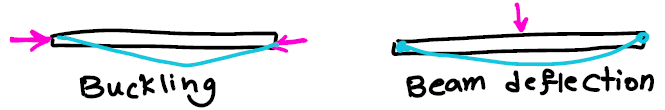
\includegraphics[angle=0, width=4in]{Buckling-Figures/BuckleVSDeflect.png}
\vspace{-2mm}
\caption{\small \blue{Taken from TAM251 Lecture Notes - L13S2}}
\vspace{-3mm}
\label{Fig:BuckVSDef}
\end{figure*}

\noindent The beam is still able to withstand normal loads, but buckling causes an \textbf{instability}. Small perturbations make the structure unstable. 

\vspace{5pt}

\noindent Failure is elastic ($\sigma < \sigma_Y$), but if increased loads are applied, further deformation and plastic failure (yielding) / brittle failure (fracture) can occur (post-buckling failure).

\subsection{\blue{Stability of Structures}}

\subsubsection{\blue{Single Column}}

\begin{figure*}[!h]
\centering
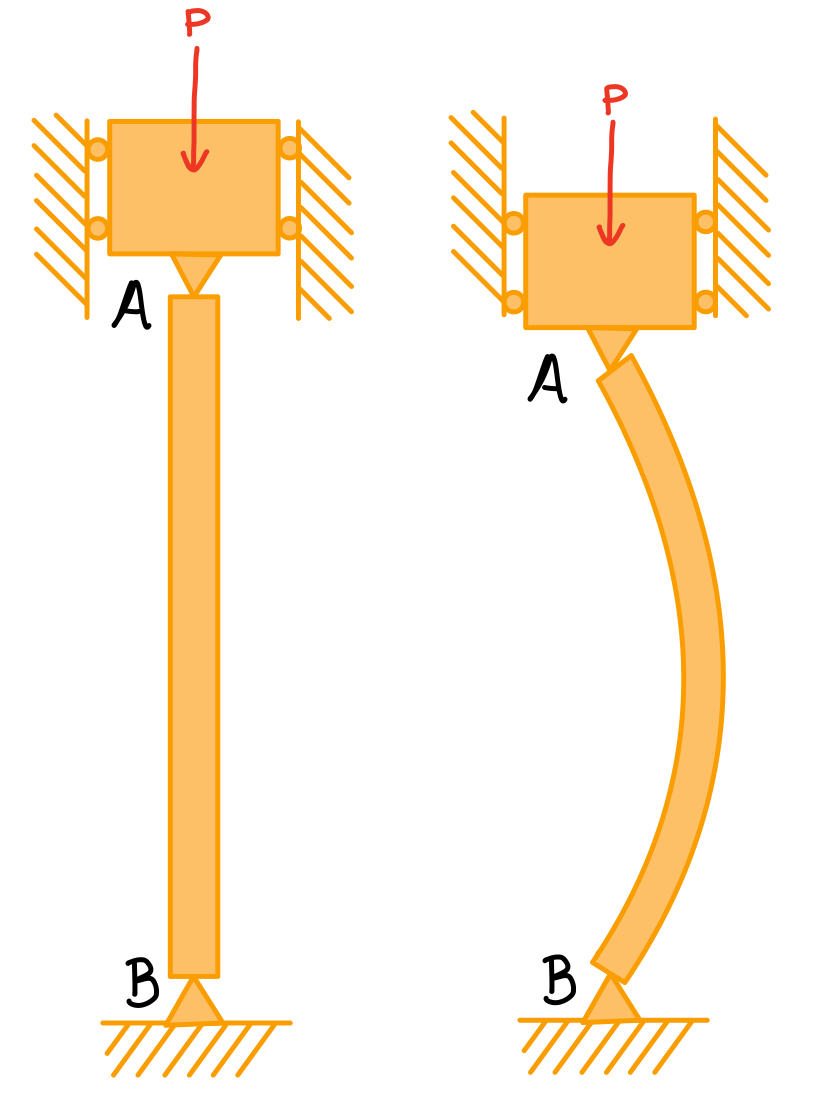
\includegraphics[angle=0, width=1.75in]{Buckling-Figures/Stability of Structures.png}
\vspace{-2mm}
\caption{\small \blue{Taken from TAM251 Lecture Notes - L13S3}}
\vspace{-3mm}
\label{Fig:Stability}
\end{figure*}

\noindent Column $AB$ is supporting uniaxial compressive load $P$. To properly design this column, the cross-section must satisfy the following:

\[\sigma = \frac{P}{A} \le \sigma_{all}\]
\[\delta = \frac{PL}{EA} \le \delta_{spec}\]

\noindent Increasing the load can cause the column to buckle $\rightarrow$ instability causing failure.

\subsubsection{\blue{Two Rods and a Torsional Spring}}

\begin{figure*}[!h]
\centering
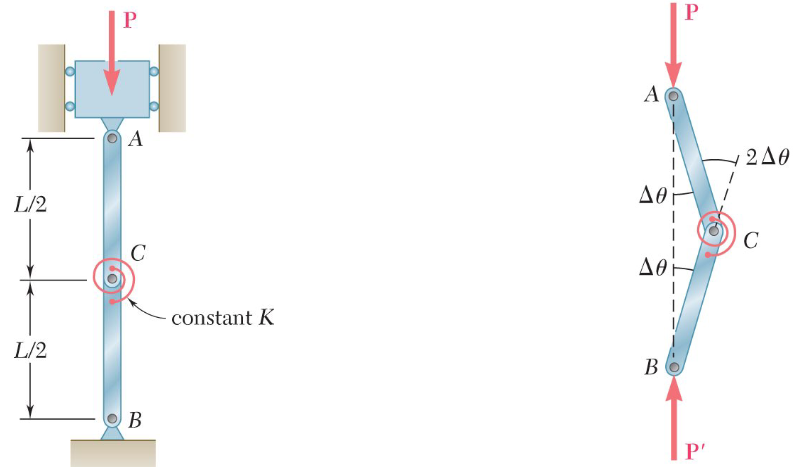
\includegraphics[angle=0, width=4in]{Buckling-Figures/TwoRods.png}
\vspace{-2mm}
\caption{\small \blue{Taken from TAM251 Lecture Notes - L13S4}}
\vspace{-3mm}
\label{Fig:TwoRods}
\end{figure*}

\noindent Rods $AC$ and $CB$ are perfectly aligned and a torsional spring connects them at point $C$. For small perturbations, point $C$ moves to the right.
\begin{itemize}
    \item If $C$ returns to the original position - the system is stable
    \item If $C$ moves farther away from the original position - the system is unstable
\end{itemize}

\begin{figure*}[!h]
\centering
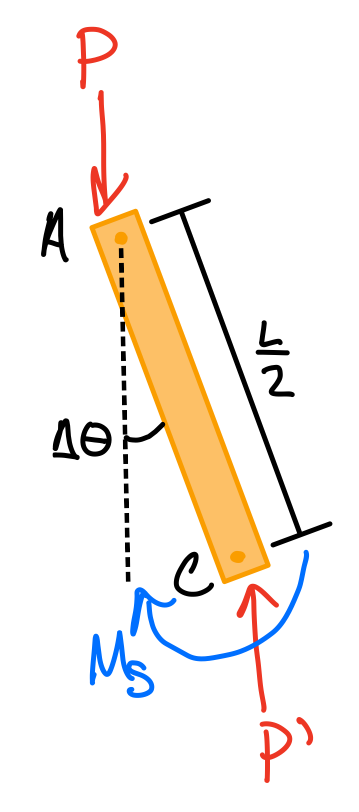
\includegraphics[angle=0, width=1in]{Buckling-Figures/TopRodFBD.png}
\vspace{-2mm}
\caption{\small \blue{Taken from TAM251 Lecture Notes - L13S5}}
\vspace{-3mm}
\label{Fig:TopRodFBD}
\end{figure*}


\noindent The spring restoring moment is 

\[M_s = K(2\Delta\theta)= \text{restoring moment}\]

\noindent The moment resultant from the applied load P tends to move the rod away from the vertical position

\[M_{load} = P\frac{L}{2}\sin\Delta\theta = P\frac{L}{2}\Delta\theta = \text{destabilizing moment}\]

\begin{itemize}
    \item Stable system: $M > M_{load}$
    \item Unstable system: $M < M_{load}$
    \item Equilibrium position gives: $M = M_{load}$
\end{itemize}

\noindent The critical load can be found with

\[P_{cr} = \frac{4K}{L}\]

\noindent \blue{\textbf{**Expandable Derivation**}}

\blue{
\[M_s = M_{load}\]
\[K(2\Delta\theta) = P_{cr}\frac{L}{2}\Delta\theta\]
}

\noindent \blue{\textbf{**End Derivation**}}


\subsection{\blue{Euler's formula}}

\blue{Euler's formula can be used to solve for the critical load of a uniaxially loaded column. 
}
\clearpage

\subsubsection{\blue{Pinned-end Columns}}

\begin{figure*}[!h]
\centering
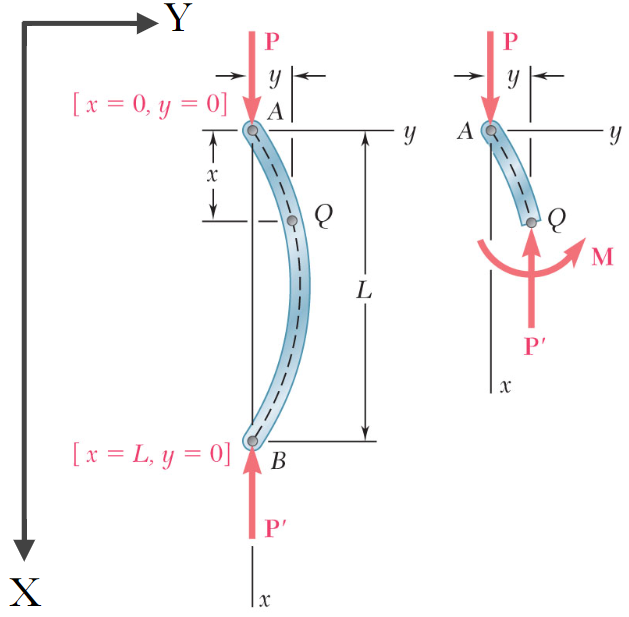
\includegraphics[angle=0, width=3in]{Buckling-Figures/Pinned.png}
\vspace{-2mm}
\caption{\small \blue{Taken from TAM251 Lecture Notes - L13S6}}
\vspace{-3mm}
\label{Fig:Pinned}
\end{figure*}

\noindent Rod $AB$ is pinned on each end.

\noindent Equilibrium gives

\[M = -Py\]

\noindent After a small perturbation, the system reaches equilibrium 


\[M(x) = EIy''(x)\]
\[EIy'' = -Py\]
\[y'' + \frac{P}{EI}y = 0\]

\noindent Linear, homogeneous differential equation of second order with constant coefficients. The general solution is 

\[y(x) = A\sin(px) + B\cos(px)\]

\noindent With boundary conditions 
\[y(0) = y(L) = 0\]

\noindent Euler's Formula 
\[P_{cr} = \frac{\pi^2EI}{L^2}\]

\noindent Buckling occurs at
\[P > P_{cr}\]

\vspace{5pt}

\noindent \blue{\textbf{**Expandable Derivation**}}

\blue{
\[y(x) = A\sin(\sqrt{\frac{P}{EI}}x) + B\cos(\sqrt{\frac{P}{EI}}x)\]
\[y(x=0)=0 \rightarrow A\sin(0)+B\cos(0) = 0\]
\[B=0\]
\[y(x=L)=0 \rightarrow A\sin(\sqrt{\frac{P}{EI}}L)+0 = 0\]
\[ A\sin(\sqrt{\frac{P}{EI}}L)=0\]
\noindent This has two solutions
}

\vspace{5pt}


\noindent \blue{(1)
\[A = 0 \rightarrow \text{not interesting}\]
}
\noindent \blue{(2)
\[A = n \rightarrow \text{ $n$: any number except where $A\sin(\sqrt{\frac{P}{EI}}L) = n\pi$ }\]
\[\frac{P}{EI}L^2 = n^2\pi^2\]
\[P_{cr} = \frac{n^2\pi^2EI}{L^2}\]
}
\noindent \blue{Buckling usually happens at the smallest non-zero value of $P_{cr}$
\[n=1\]
}
\noindent \blue{Higher $n$ values can be achieved if columns are prevented from buckling at $n=1$
}
\noindent \blue{\textbf{**End Derivation**}}

\subsubsection{\blue{Other Boundary Conditions}}

\begin{figure*}[!h]
\centering
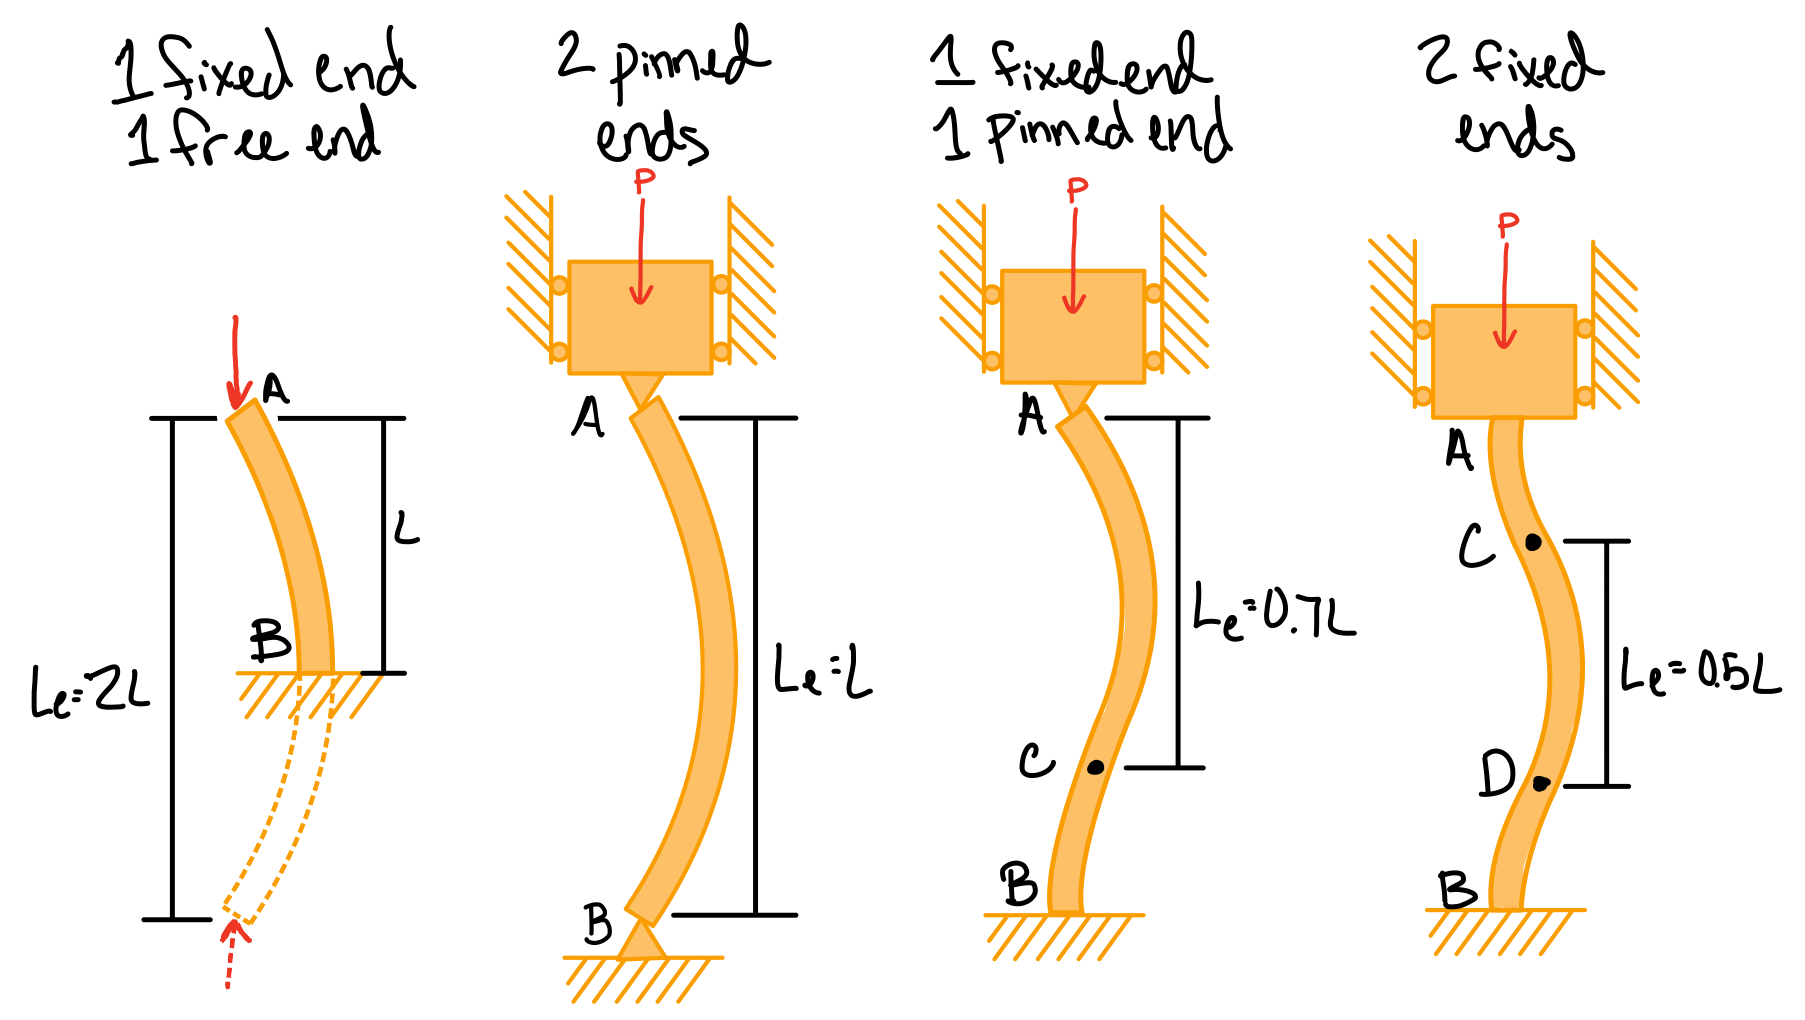
\includegraphics[angle=0, width=\columnwidth]{Buckling-Figures/EulerConditions.png}
\vspace{-2mm}
\caption{\small \blue{Taken from TAM251 Lecture Notes - L13S8}}
\vspace{-3mm}
\label{Fig:Euler}
\end{figure*}

\blue{
Different boundary conditions change length used in the critical load formula to the effective length ($L_e$).
\[P_{cr} = \frac{\pi^2EI}{L_e^2}\]
}